\documentclass[20pt]{extarticle}

\usepackage[paperwidth=36in,paperheight=48in,margin=0in]{geometry}
\usepackage[T1]{fontenc}
\usepackage{lmodern}
\usepackage{graphicx}
\usepackage{amsmath,amssymb}
\usepackage{booktabs}
\usepackage{array}
\usepackage{tabularx}
\usepackage{multirow}
\usepackage{listings}
\usepackage{tikz}
\usetikzlibrary{arrows.meta, backgrounds, calc, fit, positioning, shapes.geometric}
\usepackage{eso-pic}
\usepackage{xcolor}
\usepackage{ragged2e}
\usepackage{hyperref}

\definecolor{potsdamblue}{HTML}{00315E}
\definecolor{panelblue}{HTML}{E7F0F6}
\definecolor{lineblue}{HTML}{A9C0D5}
\definecolor{softgreen}{HTML}{EAF6EC}
\definecolor{softgold}{HTML}{FFF3D6}
\definecolor{softred}{HTML}{FBE6E6}
\definecolor{softgray}{HTML}{F6F8FA}
\definecolor{bodybg}{HTML}{F5F8FA}
\definecolor{textgray}{HTML}{1B2A34}

\setlength{\parindent}{0pt}
\setlength{\parskip}{0.35em}
\pagestyle{empty}
\color{textgray}

\lstdefinelanguage{ASP}{
  sensitive=true,
  morekeywords={not},
}

\lstset{
  language=ASP,
  basicstyle=\ttfamily\fontsize{16}{18}\selectfont,
  keywordstyle=\color{potsdamblue}\bfseries,
  frame=single,
  rulecolor=\color{lineblue},
  backgroundcolor=\color{softgray},
  columns=fullflexible,
  keepspaces=true,
  breaklines=true,
  showstringspaces=false,
  aboveskip=0.2em,
  belowskip=0.2em,
  xleftmargin=0.15in,
  xrightmargin=0.15in
}

\newsavebox{\posterboxsave}
\newlength{\posterboxwidth}
\newlength{\posterbodywidth}
\newenvironment{posterbox}[1]
  {%
    \par\noindent
    \setlength{\posterboxwidth}{\dimexpr\linewidth-2pt\relax}%
    \setlength{\posterbodywidth}{\dimexpr\posterboxwidth-0.44in\relax}%
    \begin{lrbox}{\posterboxsave}%
    \begin{minipage}{\posterboxwidth}%
      \begingroup
      \setlength{\fboxsep}{0.08in}%
      \colorbox{potsdamblue}{%
        \parbox{\dimexpr\posterboxwidth-2\fboxsep\relax}{%
          \vspace{0.03in}%
          {\color{white}\bfseries\fontsize{24}{28}\selectfont #1\par}%
          \vspace{0.02in}%
        }%
      }%
      \endgroup
      \par\vspace{0.14in}%
      \hspace*{0.22in}\begin{minipage}{\posterbodywidth}%
  }
  {%
      \end{minipage}%
      \par\vspace{0.16in}%
    \end{minipage}%
    \end{lrbox}%
    \begingroup
    \setlength{\fboxsep}{0pt}%
    \setlength{\fboxrule}{1.0pt}%
    \fcolorbox{lineblue}{white}{\usebox{\posterboxsave}}%
    \endgroup
    \par
  }

\newcommand{\sectiongap}{\vspace{0.18in}}
\newcommand{\metricvalue}[1]{{\bfseries\fontsize{32}{34}\selectfont #1}}
\newcommand{\bodytext}{\fontsize{21}{25}\selectfont}
\newcommand{\smallbody}{\fontsize{18}{21}\selectfont}
\newcommand{\tinybody}{\fontsize{16}{18}\selectfont}
\newcommand{\metriccard}[2]{%
  \begingroup
  \setlength{\fboxsep}{0.10in}%
  \setlength{\fboxrule}{0.9pt}%
  \fcolorbox{lineblue}{#1}{%
    \parbox[c][1.62in][t]{\dimexpr\linewidth-2\fboxsep-2\fboxrule\relax}{#2}%
  }%
  \endgroup
}
\newenvironment{tightitems}
  {\begin{list}{\textbullet}{%
    \setlength{\leftmargin}{0.36in}%
    \setlength{\itemsep}{0.12em}%
    \setlength{\topsep}{0.15em}%
    \setlength{\parsep}{0pt}%
    \setlength{\parskip}{0pt}}}
  {\end{list}}

\AddToShipoutPictureBG*{%
  \AtPageLowerLeft{%
    
\includegraphics[width=\paperwidth,height=\paperheight]{poster_template.pdf}%
  }%
}

\begin{document}
\bodytext

\begin{tikzpicture}[remember picture,overlay]
  % Shorten the template header while preserving its colour and logo treatment.
  \fill[potsdamblue]
    (current page.north west)
    rectangle
    ([yshift=-7.35in]current page.north east);

  \fill[bodybg]
    ([yshift=-7.35in]current page.north west)
    rectangle
    ([yshift=-9.75in]current page.north east);

  \node[anchor=north west, inner sep=0pt] at ([xshift=27.05in,yshift=-0.30in]current page.north west) {%
    
\includegraphics[
      width=6.55in,
      trim=25.5in 39.0in 1.8in 0.75in,
      clip
    ]{poster_template.pdf}%
  };

  \node[
    anchor=north west,
    text=white,
    text width=22.2in,
    align=left
  ] at ([xshift=1.50in,yshift=-0.82in]current page.north west) {%
    {\sffamily\bfseries\fontsize{84}{88}\selectfont
    LAMP: ASP Rule Induction and\\[0.08in]
    Optimization with LLMs}
  };

  \node[
    anchor=north west,
    text=white,
    align=left
  ] at ([xshift=1.58in,yshift=-4.48in]current page.north west) {%
    {\sffamily\bfseries\fontsize{48}{52}\selectfont David Bunker}\\[0.10in]
    {\sffamily\fontsize{35}{39}\selectfont University of Potsdam}
  };

  \fill[potsdamblue]
    (current page.south west)
    rectangle
    ([yshift=0.80in]current page.south east);

\end{tikzpicture}

\vspace*{7.58in}

\begin{center}
\begin{minipage}{32.6in}
\begin{posterbox}{Headline}
LAMP asks an LLM to recover ASP rules from \textit{instance facts} and an \textit{expected answer set}, then checks every candidate with \textsc{Clingo}. Across 120 synthetic rule-induction benchmarks, the strongest LAMP models nearly matched ILASP, solved every ILASP timeout case, and usually produced smaller, more stratified programs than the synthetic originals.

\vspace{0.14in}
\begin{minipage}[t]{0.238\linewidth}
\metriccard{softgreen}{%
\metricvalue{99.2\%}

Best final accuracy with LAMP\\
\textit{gpt-5-mini}: 119 / 120}
\end{minipage}\hfill
\begin{minipage}[t]{0.238\linewidth}
\metriccard{softgreen}{%
\metricvalue{98.3\%}

Best local model result\\
\textit{gpt-oss:20b}: 118 / 120}
\end{minipage}\hfill
\begin{minipage}[t]{0.238\linewidth}
\metriccard{softgold}{%
\metricvalue{3 / 3}

ILASP timeout benchmarks solved\\
by both strong LAMP models}
\end{minipage}\hfill
\begin{minipage}[t]{0.238\linewidth}
\metriccard{softgreen}{%
\metricvalue{3--6}

Average output literals for correct\\
solutions vs.\ 22 or 33 originals}
\end{minipage}
\end{posterbox}
\end{minipage}
\end{center}

\vspace{0.16in}

\begin{center}
\begin{minipage}{32.6in}
\begin{minipage}[t]{10.35in}
\vspace{0pt}
\begin{posterbox}{Problem Setting}
Writing ASP that is both correct and efficient is hard. LAMP studies a focused version of that challenge: recover a rule set from example facts and the stable model it should produce.

\[
AS(F \cup \Pi) = \{A^*\}
\]

Here $F$ is the given fact set, $A^*$ is the target answer set, $\Phi$ is a bounded hypothesis space, and the goal is to find a small program $\Pi \subseteq \Phi$ that reproduces $A^*$ exactly.

\begin{tightitems}
\item Both LAMP and ILASP receive the same facts, target answer set, and rule bounds.
\item This makes the comparison about \textit{search strategy}: LLM-guided generation versus conflict-driven symbolic search.
\item The task is intrinsically difficult: bounded-arity non-ground normal ASP reasoning is $\Sigma_2^P$-complete, and learning adds another search layer.
\end{tightitems}
\end{posterbox}

\sectiongap

\begin{posterbox}{Toy Benchmark}
\smallbody
\textbf{Facts}
\begin{lstlisting}
d0(o0).
d0(o1).
d1(o1).
\end{lstlisting}

\textbf{Target answer set}
\begin{lstlisting}
{ d0(o0), d0(o1), d1(o1), d2(o0) }
\end{lstlisting}

\textbf{One minimal solution}
\begin{lstlisting}
d2(X) :- d0(X), not d1(X).
\end{lstlisting}

\bodytext
Correctness is judged by the stable model, not by reproducing the exact synthetic source rules. Many different rule sets can yield the same answer set.
\end{posterbox}

\sectiongap

\begin{posterbox}{Benchmark Design}
\smallbody
\begin{tabular}{@{}p{4.2in}p{5.5in}@{}}
\toprule
\textbf{Parameter} & \textbf{Values used} \\
\midrule
Predicates & 6, 10 \\
Terms & 6, 10 \\
Facts & 5, 6, 9 \\
Rules & 11 \\
Overall literals & 2, 3 per rule body \\
Negative literals & 0, 1, 2 \\
Minimum derived atoms & 1, 3 \\
\bottomrule
\end{tabular}

\vspace{0.12in}
\bodytext
\begin{tightitems}
\item 120 valid synthetic combinations were generated.
\item Programs use unary predicates and normal rules only, which keeps the comparison controlled while still requiring nontrivial induction.
\item Each benchmark has exactly one answer set and at least one derived atom.
\end{tightitems}
\end{posterbox}

\sectiongap

\begin{posterbox}{Why This Matters}
\begin{tightitems}
\item ASP is powerful for configuration, planning, and combinatorial reasoning, but writing the rules is often the bottleneck.
\item The paper shows that strong current LLMs can already act as useful ASP modeling assistants when a solver is kept in the loop.
\item Because the task is rule induction rather than text translation, success here is evidence of structured reasoning rather than prompt memorization.
\end{tightitems}
\end{posterbox}

\sectiongap

\begin{posterbox}{Novelty / Positioning}
LAMP uses the LLM to generate ASP rules directly from facts, a target answer set, and rule bounds. This differs from work that uses LLMs mainly as a front end for natural-language translation or ILASP task construction. Each candidate is checked by \textsc{Clingo} at inference time, without LLM fine-tuning or ILASP-style systematic hypothesis search.
\end{posterbox}

\sectiongap

\begin{posterbox}{ILASP Baseline}
ILASP solves the same task under the Learning from Answer Sets framework, but does so with conflict-driven symbolic search over an ASP metaprogram rather than iterative LLM generation.

\begin{tightitems}
\item The hypothesis space is fixed by a mode bias derived from the benchmark profile.
\item The target answer set is encoded as a single context-dependent positive example.
\item In this study ILASP is the main symbolic baseline, run with a 420\,s timeout.
\end{tightitems}
\end{posterbox}

\sectiongap

\begin{posterbox}{Feature Analysis (RQ3)}
\smallbody
The paper also asks which benchmark features are associated with LLM failure. The strongest models missed too few cases for a useful classifier, so the analysis focuses on \textit{qwen3-coder:30b}.

\vspace{0.04in}
\centering
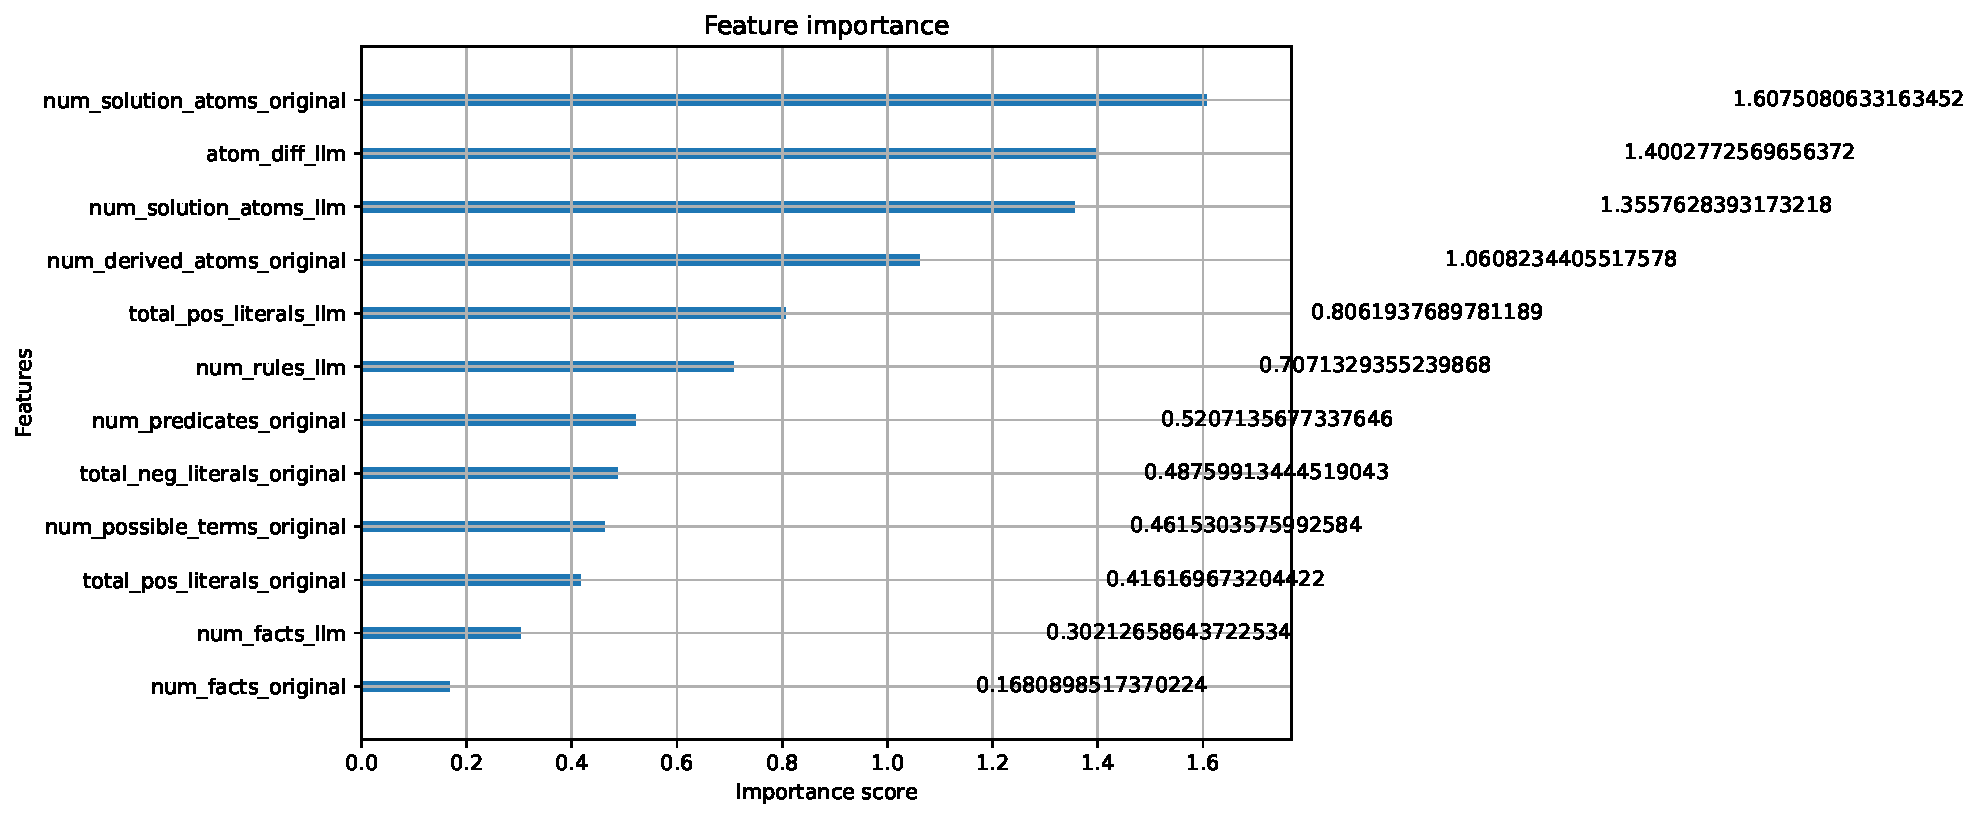
\includegraphics[width=0.72\linewidth]{../generate/diagrams/xgb_importance.pdf}

\vspace{0.06in}
\RaggedRight
The top gain features all describe scale and vocabulary breadth: larger target answer sets, more possible terms, and more predicates make exact rule recovery harder.

\vspace{0.06in}
XGBoost reached 61.7\% cross-validation accuracy with AUC 0.619, below the 64.2\% majority baseline. These are descriptive correlates, not reliable predictors yet.
\end{posterbox}
\end{minipage}\hfill
\begin{minipage}[t]{10.35in}
\vspace{0pt}
\begin{posterbox}{LAMP Protocol}
\smallbody
\begin{tightitems}
\item Prompt the LLM with instance facts $F$, target answer set $A^*$, rule schema bounds, and a worked example.
\item Parse the raw output into an ASP candidate program $\Pi_i$.
\item Run $F \cup \Pi_i$ with \textsc{Clingo}.
\item If the produced answer set mismatches $A^*$, feed the mismatch back and ask for a corrected rule set.
\item Stop after success or after 3 total attempts.
\end{tightitems}

\vspace{0.08in}
\centering
\resizebox{0.97\linewidth}{!}{%
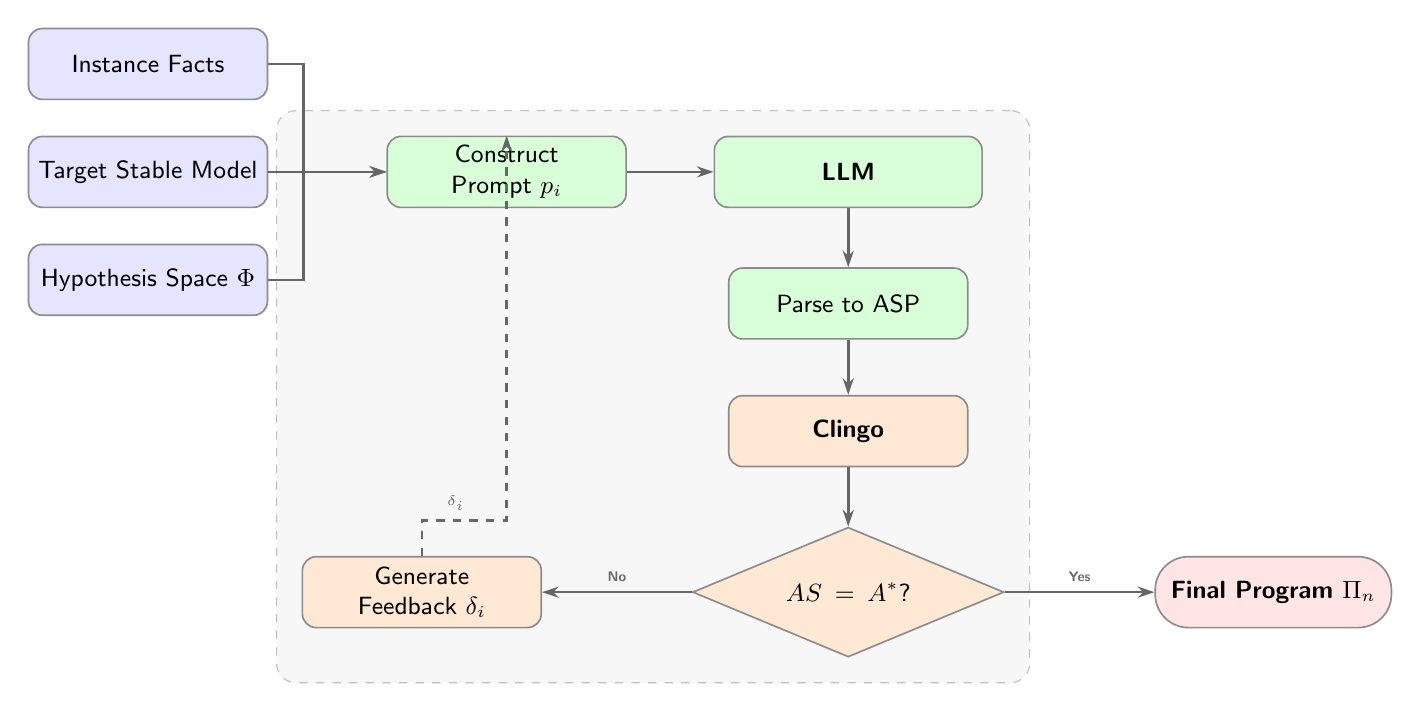
\begin{tikzpicture}[node distance=0.45cm and 1.15cm]
  \colorlet{inputcol}{blue!10}
  \colorlet{llmcol}{green!15}
  \colorlet{clingocol}{orange!17}
  \colorlet{outcol}{red!10}
  \colorlet{loopbg}{black!3}

  \tikzset{
    proc/.style={
      rectangle, rounded corners=5pt,
      minimum width=3.0cm, minimum height=0.9cm,
      text centered, text width=2.8cm,
      font=\sffamily\small,
      draw=black!45, line width=0.6pt,
      fill=#1
    },
    proc/.default=white,
    decision/.style={
      diamond, aspect=2.4,
      minimum width=3.2cm, minimum height=0.95cm,
      text centered, text width=2.6cm,
      font=\sffamily\small,
      draw=black!45, line width=0.6pt,
      fill=clingocol
    },
    terminal/.style={
      rectangle, rounded corners=12pt,
      minimum width=3.0cm, minimum height=0.9cm,
      text centered, text width=2.7cm,
      font=\sffamily\small\bfseries,
      draw=black!45, line width=0.6pt,
      fill=#1
    },
    terminal/.default=outcol,
    arr/.style={
      -{Stealth[length=6pt, width=4pt]},
      line width=0.95pt, color=black!60
    },
    darr/.style={
      -{Stealth[length=6pt, width=4pt]},
      line width=0.85pt, color=black!60, dashed
    }
  }

  \node[proc=inputcol] (facts) {Instance Facts};
  \node[proc=inputcol, below=of facts] (target) {Target Stable Model};
  \node[proc=inputcol, below=of target] (space) {Hypothesis Space $\Phi$};

  \node[proc=llmcol, right=1.5cm of target] (prompt) {Construct Prompt $p_i$};
  \node[proc=llmcol, right=1.1cm of prompt, minimum width=3.4cm] (llm) {\textbf{LLM}};
  \node[proc=llmcol, below=0.75cm of llm] (parse) {Parse to ASP};
  \node[proc=clingocol, below=0.7cm of parse] (clingo) {\textbf{Clingo}};
  \node[decision, below=0.75cm of clingo] (check) {$AS = A^*$?};
  \node[proc=clingocol, left=1.9cm of check] (feedback) {Generate Feedback $\delta_i$};
  \node[terminal=outcol, right=1.9cm of check] (out) {Final Program $\Pi_n$};

  \begin{scope}[on background layer]
    \node[draw=black!25, dashed, rounded corners=7pt, fill=loopbg,
      fit=(prompt)(llm)(parse)(clingo)(check)(feedback), inner sep=9pt] {};
  \end{scope}

  \draw[arr] (facts.east) -- ++(0.45,0) |- (prompt.west);
  \draw[arr] (target.east) -- (prompt.west);
  \draw[arr] (space.east) -- ++(0.45,0) |- (prompt.west);
  \draw[arr] (prompt.east) -- (llm.west);
  \draw[arr] (llm.south) -- (parse.north);
  \draw[arr] (parse.south) -- (clingo.north);
  \draw[arr] (clingo.south) -- (check.north);
  \draw[arr] (check.east) -- node[above, font=\sffamily\tiny\bfseries]{Yes} (out.west);
  \draw[arr] (check.west) -- node[above, font=\sffamily\tiny\bfseries]{No} (feedback.east);
  \draw[darr] (feedback.north) -- ++(0,0.45) -| node[pos=0.2, above, font=\sffamily\tiny]{$\delta_i$} (prompt.north);
\end{tikzpicture}%
}

\bodytext
The key design choice is simple: let the LLM propose rules, but let a solver decide whether those rules are actually correct.
\end{posterbox}

\sectiongap

\begin{posterbox}{Accuracy Gains From Feedback}
\smallbody
\centering
\renewcommand{\arraystretch}{1.18}
\begin{tabular}{@{}lrrr@{}}
\toprule
\textbf{System} & \textbf{1st attempt} & \textbf{Final} & \textbf{Failures} \\
\midrule
\textit{gpt-5-mini}      & 109 / 120 & 119 / 120 & 1 \\
\textit{gpt-oss:20b}     & 100 / 120 & 118 / 120 & 2 \\
\textit{qwen3-coder:30b} &  23 / 120 &  77 / 120 & 43 \\
ILASP                    & ---       & 117 / 120 & 3 \\
\bottomrule
\end{tabular}

\vspace{0.14in}
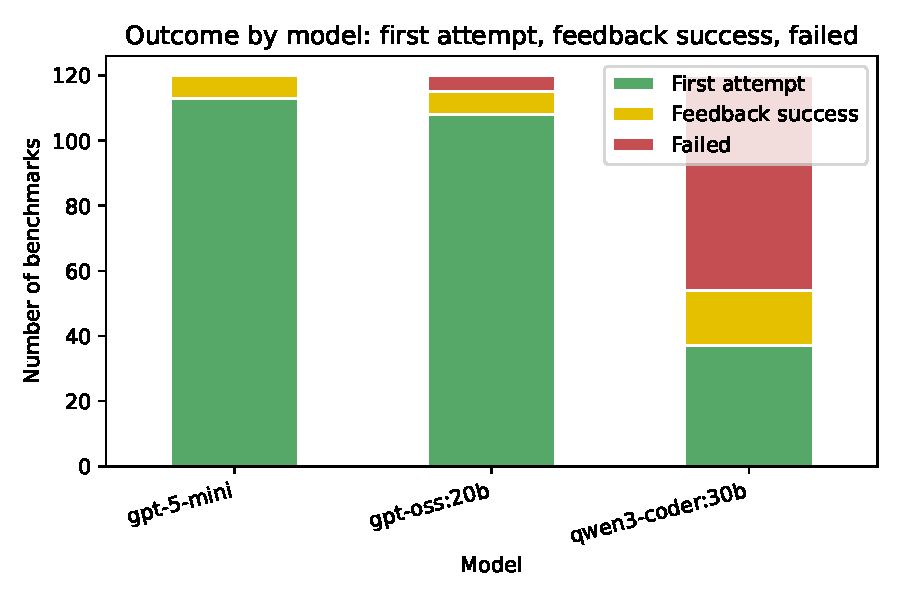
\includegraphics[width=0.96\linewidth]{../generate/diagrams/outcome_stacked.pdf}

\bodytext
Feedback recovered 10 extra cases for \textit{gpt-5-mini}, 18 for \textit{gpt-oss:20b}, and 54 for \textit{qwen3-coder:30b}. The loop matters, especially once the first draft is close but not exact.
\end{posterbox}

\sectiongap

\begin{posterbox}{Runtime And Search Behavior}
\smallbody
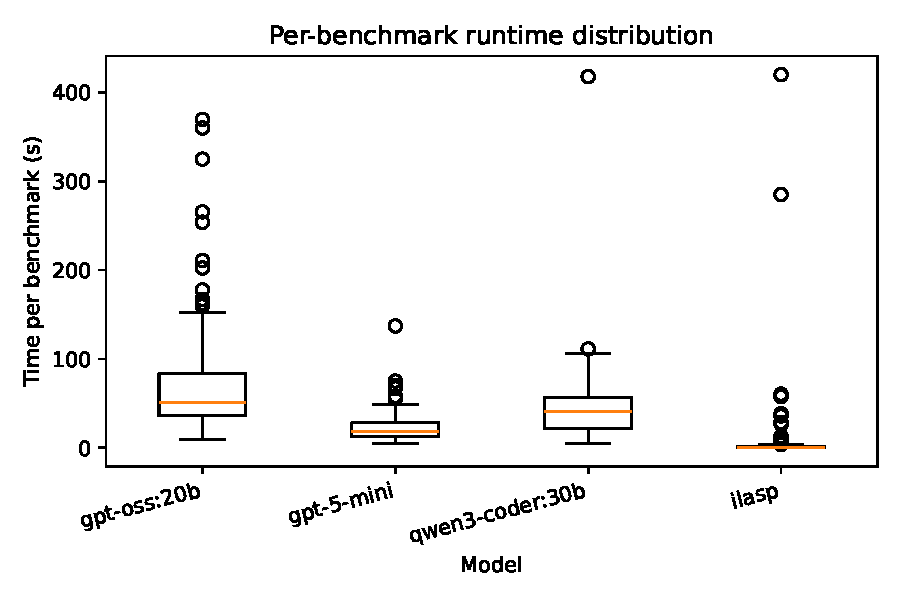
\includegraphics[width=0.96\linewidth]{../generate/diagrams/timing_boxplot.pdf}

\vspace{0.08in}
\begin{tabular}{@{}p{4.0in}p{5.55in}@{}}
\toprule
\textbf{Observation} & \textbf{Takeaway} \\
\midrule
ILASP median runtime: 0.66\,s & Conflict-driven search is usually extremely fast. \\
ILASP failures: 3, all at 420\,s & Rare search-space cliffs still matter. \\
Both strong LAMP models solved all 3 timeout cases & LLM-guided generation explores the space differently. \\
\bottomrule
\end{tabular}
\end{posterbox}

\sectiongap

\begin{posterbox}{Why Hybridize?}
\begin{tightitems}
\item ILASP gives the strong symbolic baseline: usually sub-second, concise, and principled within the mode bias.
\item LAMP is slower, but its token-level generation explores the space differently and solved all 3 ILASP timeout cases.
\item The natural next system is not LLM versus solver; it is ILASP-style search with solver-checked LLM proposals when search stalls.
\end{tightitems}
\end{posterbox}
\end{minipage}\hfill
\begin{minipage}[t]{10.35in}
\vspace{0pt}
\begin{posterbox}{Program Quality}
\smallbody
\textbf{Mean output literal count $L(\Pi)$ for correct solutions}

\vspace{0.06in}
\centering
\begin{tabular}{@{}lrrrr@{}}
\toprule
\textbf{Original} & \textbf{gpt-5} & \textbf{gpt-oss} & \textbf{qwen} & \textbf{ILASP} \\
\midrule
22 literals & 4.81 & 5.15 & 5.85 & 3.67 \\
33 literals & 3.49 & 3.82 & 3.84 & 2.71 \\
\bottomrule
\end{tabular}

\vspace{0.18in}
\textbf{Stratified solved programs}

\vspace{0.06in}
\centering
\begin{tabular}{@{}lr@{}}
\toprule
\textbf{System} & \textbf{Stratified / Solved} \\
\midrule
Original benchmarks & 49 / 120 \\
\textit{gpt-5-mini} & 119 / 119 \\
\textit{gpt-oss:20b} & 117 / 118 \\
\textit{qwen3-coder:30b} & 77 / 77 \\
ILASP & 117 / 117 \\
\bottomrule
\end{tabular}

\vspace{0.14in}
\bodytext
Both ILASP and strong LAMP models compressed the synthetic source programs heavily. Correct outputs usually needed only a handful of literals, and almost every solved program became stratified even when the original benchmark was not.
\end{posterbox}

\sectiongap

\begin{posterbox}{Timeout Cases}
\smallbody
\centering
\begin{tabular}{@{}lcccc@{}}
\toprule
\textbf{Benchmark} & \textbf{gpt-5} & \textbf{gpt-oss} & \textbf{qwen} & \textbf{ILASP} \\
\midrule
7  & \checkmark & \checkmark & $\times$ & 420\,s \\
27 & \checkmark & \checkmark & $\times$ & 420\,s \\
67 & \checkmark & \checkmark & $\times$ & 420\,s \\
\bottomrule
\end{tabular}

\vspace{0.14in}
\bodytext
The three ILASP failures were all timeouts, not logical contradictions. Each timeout case had 11 negative literals, and grounded-rule counts between 20 and 27 compared with a dataset average of 13.28. That points to search-space blowup rather than impossibility of the task.
\end{posterbox}

\sectiongap

\begin{posterbox}{What The Results Suggest}
\begin{tightitems}
\item Strong LLMs can perform nontrivial ASP rule induction even without ASP-specific training.
\item A fully local model, \textit{gpt-oss:20b}, is already close to ILASP on this benchmark class.
\item ILASP is still the faster symbolic system on average, but LAMP can succeed on some instances where exhaustive symbolic search times out.
\item The generated programs are not only correct; they are often cleaner and easier to explain than the synthetic originals.
\end{tightitems}
\end{posterbox}

\sectiongap

\begin{posterbox}{Limits And Next Steps}
\begin{tightitems}
\item The study uses synthetic benchmarks with unary predicates, normal rules, and exactly one answer set.
\item Each model was run once per benchmark at temperature 1, so small score gaps should be interpreted cautiously.
\item Richer targets include higher-arity ASP, choice rules, disjunction, aggregates, planning benchmarks, and ASPBench.
\item The most interesting extension is a hybrid system: ILASP-style search plus an agentic LLM refinement loop.
\end{tightitems}
\end{posterbox}

\sectiongap

\begin{posterbox}{Experimental Controls}
\smallbody
\begin{tightitems}
\item Same input instance for both systems: facts, target answer set, and bounded rule schema.
\item LAMP uses 3 total attempts: one initial generation and up to 2 solver-feedback rounds.
\item All LLMs were run once per benchmark at temperature 1.
\item \textit{gpt-5-mini} used the OpenAI API; \textit{gpt-oss:20b} and \textit{qwen3-coder:30b} ran locally with Ollama.
\item ILASP version 4 and all LAMP runs used the same 420\,s timeout.
\item A LAMP output only counts as correct when \textsc{Clingo} returns exactly the target stable model.
\end{tightitems}

\vspace{0.08in}
\tinybody
Source code, benchmark data, and generated ILASP tasks: \url{https://github.com/dbunker/lamp}.
\end{posterbox}

\sectiongap

\begin{posterbox}{Research Questions Answered}
\smallbody
\begin{tabular}{@{}p{1.1in}p{8.35in}@{}}
\textbf{RQ1} & Yes: solver-in-the-loop prompting can produce correct ASP encodings from facts and a target answer set. \\
\textbf{RQ2} & LAMP nearly matches ILASP in accuracy; ILASP is faster on average, but LAMP solves the ILASP timeout cases. \\
\textbf{RQ3} & Failure correlates mostly with target size and vocabulary breadth, but the current sample is too small for reliable prediction. \\
\end{tabular}
\end{posterbox}

\sectiongap

\begin{posterbox}{Take-home}
{\bfseries Solver-in-the-loop prompting makes ASP rule induction practical.}
ILASP remains the fast symbolic baseline, but LAMP provides a complementary LLM-guided search strategy: it nearly matches ILASP overall, solves the ILASP timeout cases, and often returns compact, stratified programs.
\end{posterbox}
\end{minipage}
\end{minipage}
\end{center}

\end{document}
